\section{Replication details and source versions}
\label{app:replication}

This study replicates and extends the empirical framework of \citet{greenwood2025} in Sweden. The detailed comparison uses their March 2024 author manuscript, deposited in Harvard DASH under the 2025 publication record \citep{greenwood2024ms}. That manuscript is not authenticated as the final published text: its abstract reports a recent deletion return of 0.1\%, while its body retains an older estimate of $-0.6$\%. Published headline comparisons therefore use the journal's abstract; the method references below identify the March 2024 version explicitly. The published full text and official replication files were not accessible for this review, leaving program-level equivalence unresolved.

The author manuscript's Equation~(2) defines excess cumulative stock returns relative to the S\&P~500 over announcement, implementation and announcement-to-implementation windows. Its Equation~(1) motivates a price multiplier $M$ applied to measured demand $D$. The Swedish analysis preserves these organizing questions, replacing the benchmark with OMXSBGI. It adapts the event screens, investor classifications, reporting intervals and inference to the available Swedish data. In particular, review clustering differs from the White standard errors in the original main tables; many Swedish securities change membership simultaneously.

\begin{table}[H]
\centering
\caption{From Greenwood--Sammon to the Swedish implementation}\label{tab:replication_map}
\small
\setlength{\tabcolsep}{5pt}
\begin{tabular}{p{2.0cm}p{4.65cm}p{6.1cm}}
\toprule
Component & Anchor study & Swedish analysis \\
\midrule
Return pattern & S\&P 500 additions/deletions; announcement, implementation and full windows & OMXSB; same event-window questions, explicitly defined daily-sum CAR \\
Time comparison & Long US history and decade means & Four Swedish calendar blocks and two pooled decades; incomplete 2026 \\
Composition & Period indicators and four firm characteristics & Same regression structure; Swedish measurement proxies and common samples \\
Index demand & Tracking-trade classification; quarterly holdings & Dated mandate groups; available pre/post reports; FI comparison \\
Other index activity & Migrations within S\&P index families & Coincident MSCI changes; a distinct overlap diagnostic \\
Anticipation & Pre-announcement returns and longer starting window & Pre-return windows and AD-20 to ED+1 ratio; historical eligibility not fully reconstructed \\
Liquidity & Effective spreads and implementation costs & Closing quoted spreads and daily volume concentration \\
Extensions & Anchor comparison provides the baseline & Fixed-duration timing, within-firm share classes and separate holdings reporting \\
\bottomrule
\end{tabular}
\begin{minipage}{\linewidth}\footnotesize\vspace{5pt}
The mapping distinguishes conceptual replication from exact numerical reproduction. Detailed source-version references and adaptations appear in Appendix~\ref{app:replication}. Differences in periods, sample selection, holdings dates and return conventions prevent interpreting raw cross-country differences as causal effects.
\end{minipage}
\end{table}


The US tracker classification uses the average annual share of index trades and a 50\% threshold. Swedish production estimates instead use curated, dated fund classifications. The US observations straddle quarterly reports, while Swedish snapshots are sought before AD and after ED. The original acquisition and listing screens also differ from the Swedish offer/delisting exclusions. These departures preclude describing the exercise as an exact reproduction. Likewise, MSCI overlap is a concurrent-event sensitivity, not a reconstruction of the original S\&P index-family migration mechanism.

The four composition controls retain the original categories: abnormal turnover, relative size, residual variance and analyst coverage. Their construction is adapted: the Swedish monthly forecast count need not equal the original unique-analyst count at the latest earnings announcement. Demand also uses ED shares outstanding rather than the original post-event quarterly denominator. The multiplier with controls scales period indicators by period-average demand; it is not an event-level regression of returns on individual fund purchases.

The pre-announcement exercise follows the original paper's anticipation question, but positive prior returns can also reflect selection on performance. The longer demand-ratio window is AD$-20$ through ED$+1$, as in the author manuscript's Tables~5--6. It should be distinguished from the separate Swedish extension through ED$+20$.

\begin{table}[!htbp]
\centering
\caption{The earlier-start demand-ratio window}\label{tab:long_demand}
\small
\setlength{\tabcolsep}{5pt}
\begin{tabular}{llrrrr}
\toprule
Type & Period & Short $N$ & Short $M$ & Long $N$ & Long $M$ \\
\midrule
Addition & 2007--11 & 8 & 57.87 & 8 & 60.83 \\
Addition & 2012--16 & 27 & -3.76 & 27 & -1.82 \\
Addition & 2017--21 & 58 & 2.97 & 58 & 4.24 \\
Addition & 2022--26 & 78 & 2.35 & 75 & 6.66 \\
Deletion & 2007--11 & 7 & -0.72 & 7 & 12.98 \\
Deletion & 2012--16 & 25 & 4.36 & 25 & 8.49 \\
Deletion & 2017--21 & 40 & 0.20 & 40 & -0.57 \\
Deletion & 2022--26 & 68 & 1.41 & 67 & 2.44 \\
\bottomrule
\end{tabular}
\begin{minipage}{\linewidth}\footnotesize\vspace{5pt}
Short is AD-1 to ED+1; Long is AD-20 to ED+1, the earlier-start counterpart in the anchor study. Each ratio uses identical events in its own numerator and denominator, but the short and long samples can differ. These are descriptive point estimates; the table does not claim well-identified early multipliers. The ED+20 analysis is a separate extension.
\end{minipage}
\end{table}

\FloatBarrier

\section{Return conventions and source checks}
\label{app:data}
\label{app:definitions}

\begin{table}[!htbp]
\centering
\caption{Coverage across periods}\label{tab:sample_by_period}
\small
\setlength{\tabcolsep}{5pt}
\begin{tabular}{llrrrr}
\toprule
Type & Period & Source events & Return sample & Holdings sample & Reviews \\
\midrule
Addition & 2007--2011 & 48 & 33 & 8 & 9 \\
Addition & 2012--2016 & 58 & 54 & 27 & 10 \\
Addition & 2017--2021 & 90 & 82 & 58 & 10 \\
Addition & 2022--2026 & 88 & 87 & 78 & 9 \\
Deletion & 2007--2011 & 54 & 33 & 7 & 9 \\
Deletion & 2012--2016 & 53 & 46 & 25 & 10 \\
Deletion & 2017--2021 & 66 & 61 & 40 & 10 \\
Deletion & 2022--2026 & 79 & 75 & 68 & 9 \\
\bottomrule
\end{tabular}
\begin{minipage}{\linewidth}\footnotesize\vspace{5pt}
The source inventory precedes security matching, exclusions and return requirements. Return sample requires complete AD-1 through ED+1 returns after the stated deletion exclusions. Holdings sample additionally requires the broad demand measure and retention under the share-adjustment screen, with a nonmissing matching return. Reviews counts distinct review cycles in the return sample. The figures describe coverage, not random attrition.
\end{minipage}
\end{table}


The observation is a security--review event; an issuer can recur or contribute different share classes. Dates are mapped to the observed trading calendar. Every stated CAR window includes the daily returns at both endpoints. Thus AD$-1$ is the first included daily return, not the closing-price baseline for the subsequent investment. CAR sums daily percentage stock returns less daily OMXSBGI returns. Stock total returns are used where available, with closing-price returns as a fallback. This convention does not automatically preserve dividends in every fallback observation.

The source manuscript calls its inputs cumulative returns but does not settle the daily aggregation or endpoint conventions sufficiently to authenticate an exact match. Table~\ref{tab:return_conventions} therefore compares arithmetic sums with compounded stock returns minus compounded benchmark returns on identical observations and included days. For 2017--2026 additions, the means are 2.15\% and 2.18\%; in 2022--2026 they are 1.50\% and 1.45\%. Interpreting AD$-1$ as a baseline close instead changes the later-decade mean to approximately 2.75\%. That is a change of included returns, not a compounding result.

\begin{table}[!htbp]
\centering
\caption{Return definitions on matched events}\label{tab:return_conventions}
\small
\setlength{\tabcolsep}{5pt}
\begin{tabular}{llrrrr}
\toprule
Type & Period & Events & Daily sum & Compounded & Base at AD-1 \\
\midrule
Addition & 2007--2011 & 33 & 8.52 & 8.60 & 9.27 \\
Addition & 2012--2016 & 54 & 0.25 & 0.38 & 0.42 \\
Addition & 2017--2021 & 82 & 2.85 & 2.96 & 4.20 \\
Addition & 2022--2026 & 87 & 1.50 & 1.45 & 1.38 \\
Addition & 2017--2026 & 169 & 2.15 & 2.18 & 2.75 \\
Deletion & 2007--2011 & 33 & -6.16 & -6.05 & -6.61 \\
Deletion & 2012--2016 & 46 & -2.47 & -2.38 & -2.62 \\
Deletion & 2017--2021 & 61 & -0.43 & -0.53 & -0.37 \\
Deletion & 2022--2026 & 75 & -1.53 & -1.63 & -1.87 \\
Deletion & 2017--2026 & 136 & -1.04 & -1.14 & -1.20 \\
\bottomrule
\end{tabular}
\begin{minipage}{\linewidth}\footnotesize\vspace{5pt}
Daily sum is the primary arithmetic CAR. Compounded is the stock buy-and-hold return minus the benchmark buy-and-hold return using the same included daily returns, AD-1 through ED+1. Base at AD-1 instead starts from the AD-1 close and includes daily returns AD through ED+1. Both latter columns compound stock and benchmark separately. These are sensitivity checks, not proof of the original US code\textquotesingle{}s convention.
\end{minipage}
\end{table}


The announcement-to-effective lag ranges from six to eighteen trading days. It is generally fourteen to eighteen days during 2010--2019 and six to eight days during 2022--2026. Consequently, the total event window changes duration. The common AD$-1$ through AD$+5$ sensitivity ends before ED in every review; its complement begins at AD$+6$. Their sum exactly recovers the total CAR on the same cohort. The first-to-last addition decline is concentrated in this remainder, whose duration and composition also vary. This accounting does not show that shorter notice caused lower returns.

External research recovered accessible notices or original attachments for 35 of 39 reviews, sometimes through republication; three further reviews were visible only in indexed text. The 2008 second-half notice remained unresolved. A December 2008 correction also prints an inconsistent effective year. Document retrieval is not complete field-level reconciliation, and neither a trading-volume peak nor the label ``effective date'' independently authenticates open-versus-close implementation conventions.
\FloatBarrier

\section{Holdings measurement and coverage}
\label{app:holdings}

Group C combines strict followers, benchmark variants and funds with an OMXSB-linked component. It measures covered positions rather than all passive capital. The numerator reconstructs to numerical precision for all 311 complete primary holdings events. Available timestamps satisfy the stated pre-AD and post-ED limits, but this verifies recorded dates rather than the completeness of the underlying reports. Forty fund-event records use a pre-position date different from the latest fund report identified by the availability check.

An absent position is treated as zero when other reporting establishes fund availability. Among addition records, 1,630 of 1,739 contributing fund-event observations have no observed pre-position row. A zero is plausible for a newly included security, but a security-query extract cannot independently distinguish it from an omitted response. Original reports or vendor completeness information are required to resolve that distinction.

The adjustment exclusion compares a market-capitalization/share-count/adjusted-price proxy at ED with its value at the security's final available price date. A missing ratio or a ratio outside $[1/1.4,1.4]$ triggers exclusion. It is therefore a share-adjustment consistency screen, not simply a record of splits during the event window. Later corporate actions can affect early-event eligibility. This safeguard may be needed because adjusted fund shares are divided by historical shares outstanding; removing it without reconciling vendor conventions would not be a justified correction.

\begin{table}[!htbp]
\centering
\caption{Fund definitions on the broad-measure event sample}\label{tab:holdings_coverage}
\small
\setlength{\tabcolsep}{5pt}
\begin{tabular}{llrrrrr}
\toprule
Type & Period & Events & Strict & + variants & Broad & Mixed count \\
\midrule
Addition & 2007--11 & 8 & 0.10 & 0.15 & 0.15 & 0.0 \\
Addition & 2012--16 & 27 & 0.37 & 0.49 & 0.52 & 0.4 \\
Addition & 2017--21 & 58 & 0.92 & 1.02 & 1.11 & 1.0 \\
Addition & 2022--26 & 78 & 0.41 & 0.78 & 0.97 & 8.8 \\
Deletion & 2007--11 & 7 & 0.20 & 0.26 & 0.26 & 0.0 \\
Deletion & 2012--16 & 25 & 0.31 & 0.46 & 0.48 & 0.1 \\
Deletion & 2017--21 & 40 & 0.83 & 0.92 & 0.99 & 1.0 \\
Deletion & 2022--26 & 68 & 0.52 & 0.93 & 1.18 & 9.4 \\
\bottomrule
\end{tabular}
\begin{minipage}{\linewidth}\footnotesize\vspace{5pt}
Demand is percent of shares outstanding, sign-adjusted for deletions. All three demand definitions in a row use the same retained event sample. Strict comprises exact benchmark followers; the next column adds related benchmark variants; Broad also includes the benchmark-linked mixed-fund category. Mixed count is the mean number of reporting mixed funds per event, not their ownership percentage. These data do not measure the complete investor universe.
\end{minipage}
\end{table}


All 468 stored share denominators and adjustment ratios reconstruct. For the 311 retained holdings observations, the denominator exists on ED in the daily panel, although daily availability does not prove that the underlying issuer disclosure is fresh. The screen removes 26 of 37 early addition candidates, compared with nine of 87 in the latest block, contributing to unequal historical coverage.

A fixed-universe sensitivity intersects verified mandate status and reporting availability across every review, without selecting on purchases or returns. No fund survives all 39 reviews. Three survive the 19 later reviews: Swedbank Robur Access Mix, Swedbank Robur Access Sverige and iShares OMX Stockholm Capped UCITS ETF. Within each block, on the same additions as the broad measure, their mean purchases fall from 0.488\% to 0.378\% between the last two blocks, compared with 1.107\% and 0.973\% for broad C. The narrower measure retains the same missing-position assumptions and omits relevant investors. It supports neither continuously increasing purchases nor a corrected estimate of total index demand.
\FloatBarrier

\section{Statistical inference and sensitivity}
\label{app:inference}

For the event-weighted mean $\widehat\mu=N^{-1}\sum_i y_i$, review-clustered CR1 variance is
\begin{equation}
 \widehat V(\widehat\mu)=\frac{G}{G-1}\frac{1}{N^2}
 \sum_{g=1}^G\left[\sum_{i\in g}(y_i-\widehat\mu)\right]^2,
\end{equation}
where $G$ is the number of reviews. The intercept-only regression's remaining degrees-of-freedom correction equals one. Joint covariance of mean signed returns and demand uses the corresponding two-dimensional review scores.

For the ratio $\widehat M=\overline Y/\overline D$, a candidate value $m$ belongs to the Fieller set if
\begin{equation}
 (\overline Y-m\overline D)^2\leq
 t_{G-1,0.975}^{2}
 \left[\widehat V_{YY}-2m\widehat V_{YD}+m^2\widehat V_{DD}\right].
 \label{eq:fieller}
\end{equation}
This accounts for covariance between numerator and denominator \citep{fieller1954}. Sets can be bounded, unbounded or all real values; weak denominator precision must not be concealed by discarding inconvenient outcomes. With few reviews, the approximation does not guarantee exact coverage. The early addition set spans $[-9.55,471.88]$, while the earliest deletion set contains every real value. These estimates cannot establish a precise historical change in structural elasticity.

\begin{table}[!htbp]
\centering
\caption{Returns scaled by observed benchmark linked fund purchases}\label{tab:demand}
\small
\setlength{\tabcolsep}{5pt}
\begin{tabular}{llrrrrrl}
\toprule
Type & Period & $N$ & $G$ & $\bar Y$ & $\bar D_C$ & $\widehat M$ & Fieller set \\
\midrule
Addition & 2007--11 & 8 & 5 & 8.78 & 0.15 & 57.87 & [-9.55, 471.88] \\
Addition & 2012--16 & 27 & 8 & -1.94 & 0.52 & -3.76 & [-15.09, 4.24] \\
Addition & 2017--21 & 58 & 10 & 3.29 & 1.11 & 2.97 & [-0.14, 6.30] \\
Addition & 2022--26 & 78 & 9 & 2.28 & 0.97 & 2.35 & [-0.21, 4.73] \\
Addition & 2017--26 & 136 & 19 & 2.71 & 1.03 & 2.63 & [0.91, 4.37] \\
Deletion & 2007--11 & 7 & 3 & -0.19 & 0.26 & -0.72 & All real values \\
Deletion & 2012--16 & 25 & 7 & 2.07 & 0.48 & 4.36 & [-17.73, 30.17] \\
Deletion & 2017--21 & 40 & 10 & 0.20 & 0.99 & 0.20 & [-4.05, 4.89] \\
Deletion & 2022--26 & 68 & 9 & 1.66 & 1.18 & 1.41 & [-0.87, 2.83] \\
Deletion & 2017--26 & 108 & 19 & 1.12 & 1.11 & 1.01 & [-0.88, 2.61] \\
\bottomrule
\end{tabular}
\begin{minipage}{\linewidth}\footnotesize\vspace{5pt}
$Y=s_i CAR_i[AD-1,ED+1]$ and $D_C$ is the sign-adjusted change in covered benchmark-linked funds\textquotesingle{} holdings as a percentage of shares outstanding; $s_i=1$ for additions and $-1$ for deletions. Positive values therefore indicate movement in the index-directed direction for both event types. $\widehat M=\bar Y/\bar D_C$ uses the same adjustment-screened complete-case sample for both means. Group C includes strict followers, benchmark variants, and benchmark-linked mixed-fund holdings. The last column is a 95\% Fieller confidence set using the joint CR1 covariance of both means and $t_{G-1}$, an asymptotic sensitivity measure rather than exact small-sample inference. It differs from the percentile bootstrap. Source: Authors' calculations; exact inputs are listed in the replication package.
\end{minipage}
\end{table}


\subsection{Weighting and dependence}
\label{app:dependence}
\begin{table}[!htbp]
\centering
\caption{Weighting and dependence sensitivity}\label{tab:dependence}
\small
\setlength{\tabcolsep}{5pt}
\begin{tabular}{llrrlrrr}
\toprule
Type & Period & Event & Review & Leave one out & CR1 & CV3 & Two way \\
\midrule
Addition & 2017--2026 & 2.15 & 2.50 & [1.87, 2.47] & 0.55 & 0.55 & 0.47 \\
Addition & 2022--2026 & 1.50 & 1.50 & [1.02, 2.01] & 0.74 & 0.77 & 0.71 \\
Deletion & 2017--2026 & -1.04 & -0.52 & [-1.45, -0.50] & 0.87 & 0.88 & 0.87 \\
Deletion & 2022--2026 & -1.53 & -1.32 & [-2.06, -0.58] & 1.12 & 1.17 & 1.11 \\
\bottomrule
\end{tabular}
\begin{minipage}{\linewidth}\footnotesize\vspace{5pt}
CAR $[AD-1,ED+1]$ in percent. Review mean gives each review equal weight. Leave one out is the range of event-weighted estimates after removing one review at a time, not a confidence interval. CR1, CV3 and Two way report standard errors. CV3 is the cluster jackknife centered on the full-sample estimate. Two way combines review and security clustering with subtraction of the review-security intersection. It does not solve dependence between different securities across different reviews. Source: Authors' calculations; exact inputs are listed in the replication package.
\end{minipage}
\end{table}


Equal-event and equal-review means answer different averaging questions. Leave-one-review-out ranges describe influence rather than confidence coverage. The jackknife and review-by-security covariance checks address additional dependence assumptions; two-way clustering does not capture every correlation across different securities and reviews \citep{petersen2009,cameron2011,mackinnon2023}.

\begin{table}[!htbp]
\centering
\caption{Changes in the event window return}\label{tab:contrasts}
\small
\setlength{\tabcolsep}{5pt}
\begin{tabular}{lllrr}
\toprule
Type & Contrast & Estimate & 95\% interval & $p$ \\
\midrule
Addition & Latest minus earliest & -7.03 & [-13.10, -1.10] & 0.029 \\
Addition & Latest minus preceding & -1.35 & [-3.88, 0.98] & 0.250 \\
Addition & Later minus earlier decade & -1.24 & [-5.26, 2.54] & 0.502 \\
Addition & Linear trend per year & -0.28 & [-0.64, 0.08] & 0.117 \\
Deletion & Latest minus earliest & 4.62 & [0.25, 9.81] & 0.039 \\
Deletion & Latest minus preceding & -1.10 & [-5.11, 2.70] & 0.564 \\
Deletion & Later minus earlier decade & 2.97 & [-2.94, 8.60] & 0.328 \\
Deletion & Linear trend per year & 0.19 & [-0.29, 0.64] & 0.400 \\
\bottomrule
\end{tabular}
\begin{minipage}{\linewidth}\footnotesize\vspace{5pt}
The outcome is CAR $[AD-1,ED+1]$. Differences are percentage points; the linear trend is percentage points per calendar year. Earliest, preceding, and latest periods are 2007--2011, 2017--2021, and 2022--2026. Decades are 2007--2016 and 2017--2026. Restricted wild bootstrap inference clusters by review cycle, using 9,999 draws. A difference of significance levels across periods is not a test of a difference. Source: Authors' calculations; exact inputs are listed in the replication package.
\end{minipage}
\end{table}


\subsection{Multiplicity, equivalence and precision}
\label{app:multi}
\begin{table}[!htbp]
\centering
\caption{Multiplicity in a declared ten test audit family}\label{tab:multiplicity}
\small
\setlength{\tabcolsep}{5pt}
\begin{tabular}{llrr}
\toprule
Type & Test & Raw $p$ & Holm $p$ \\
\midrule
Addition & 2007--2011 & 0.027 & 0.214 \\
Addition & 2012--2016 & 0.908 & 1.000 \\
Addition & 2017--2021 & 0.005 & 0.046 \\
Addition & 2022--2026 & 0.062 & 0.310 \\
Addition & 2022--26 minus 2007--11 & 0.029 & 0.214 \\
Deletion & 2007--2011 & 0.007 & 0.059 \\
Deletion & 2012--2016 & 0.522 & 1.000 \\
Deletion & 2017--2021 & 0.759 & 1.000 \\
Deletion & 2022--2026 & 0.279 & 1.000 \\
Deletion & 2022--26 minus 2007--11 & 0.039 & 0.235 \\
\bottomrule
\end{tabular}
\begin{minipage}{\linewidth}\footnotesize\vspace{5pt}
The audit family contains eight five-year total-window means and two latest-minus-earliest contrasts. It was declared after the results were known. Holm adjustment controls familywise error for this family under valid marginal tests; it cannot correct unrecorded historical specification search. It does not turn the thesis into a preregistered study. Source: Authors' calculations; exact inputs are listed in the replication package.
\end{minipage}
\end{table}


Only the 2017--2021 addition mean remains below 0.05 after Holm adjustment within the declared ten-test family \citep{holm1979}. That family was specified after inherited results were known and excludes many historical specifications. It is a limited sensitivity, not a retrospective confirmatory design.

The archived minimum-detectable-effect approximation is
\begin{equation}
 MDE\approx\left(t_{G-1,0.975}+t_{G-1,0.80}\right)\widehat{SE}.
 \label{eq:mde}
\end{equation}
It describes the scale associated with an approximate two-sided 5\% test at 80\% power, not exact bootstrap power. The latest addition MDE is 2.35 percentage points. Its analytical 90\% interval, $[0.13,2.87]$, does not establish equivalence within the illustrative $\pm1$ percentage-point margin; neither does the deletion interval $[-3.62,0.55]$. The margin was chosen after existing results were known.

\subsection{Timing and longer-horizon checks}
\label{app:horizon}
\begin{table}[!htbp]
\centering
\caption{First-to-last changes in the timing decomposition}\label{tab:timing_contrasts}
\small
\setlength{\tabcolsep}{5pt}
\begin{tabular}{lllrl}
\toprule
Type & Component & Difference & 95\% CR1 interval & $p$ \\
\midrule
Addition & Full window & -7.03 & [-11.97, -2.08] & 0.027 \\
Addition & Initial seven days & 0.62 & [-1.80, 3.03] & 0.625 \\
Addition & Remaining interval & -7.64 & [-11.91, -3.37] & 0.009 \\
Deletion & Full window & 4.62 & [0.38, 8.87] & 0.040 \\
Deletion & Initial seven days & 2.78 & [-0.10, 5.66] & 0.088 \\
Deletion & Remaining interval & 1.84 & [-2.35, 6.04] & 0.404 \\
\bottomrule
\end{tabular}
\begin{minipage}{\linewidth}\footnotesize\vspace{5pt}
Differences are 2022--2026 minus 2007--2011, in percentage points, from a four-period indicator regression. Intervals are analytical CR1 using review clusters; two-sided tests use 49,999 restricted wild draws. These are pointwise exploratory tests, not adjusted for all prior specification choices. The component contrasts add to the full contrast.
\end{minipage}
\end{table}

\begin{table}[!htbp]
\centering
\caption{Exclusions in the exploratory cumulative return extension}\label{tab:horizon_checks}
\small
\setlength{\tabcolsep}{5pt}
\begin{tabular}{llrrlr}
\toprule
Period & Sample & $N$ & CAR & CR1 interval & $p_{WCR}$ \\
\midrule
2017--2026 & full & 169 & 3.30 & [1.31, 5.28] & $<0.001$ \\
2017--2026 & without Sivers & 168 & 3.07 & [0.96, 5.18] & 0.003 \\
2017--2026 & without MSCI overlap & 157 & 2.51 & [0.60, 4.42] & 0.008 \\
2017--2026 & without screened company news & 163 & 3.14 & [1.13, 5.15] & $<0.001$ \\
2022--2026 & full & 87 & 1.71 & [0.72, 2.69] & 0.010 \\
2022--2026 & without Sivers & 86 & 1.25 & [-0.14, 2.63] & 0.087 \\
2022--2026 & without MSCI overlap & 82 & 1.21 & [-0.25, 2.67] & 0.114 \\
2022--2026 & without screened company news & 84 & 1.79 & [1.04, 2.53] & 0.003 \\
\bottomrule
\end{tabular}
\begin{minipage}{\linewidth}\footnotesize\vspace{5pt}
CAR $[AD-1,ED+20]$ in percent, constructed on complete non-overlapping before/after cohorts. Each exclusion is separate. These follow-up diagnostics were added after inspecting the new cumulative estimates, and inherit the limitations of the original screens. Analytical intervals and 49,999-draw wild-bootstrap $p$-values have the same definitions as Table \ref{tab:horizon_main}. Source: Authors' calculations; exact inputs are listed in the replication package.
\end{minipage}
\end{table}


The fixed-window decomposition and ED$+20$ extension are exploratory. New analytical intervals use CR1 and $t_{G-1}$, while separately reported restricted wild-bootstrap tests use 49,999 draws and finite-simulation correction. They are not inverted versions of those intervals. News and concurrent-index exclusions change the sample and remain incomplete. A positive cumulative return through ED$+20$ neither establishes permanent impact nor proves positive post-effective drift. All periods and both event types are retained in the supporting outputs.
\FloatBarrier

\section{Repaired comparison-security estimates}
\label{app:comparisons}
\begin{table}[!htbp]
\centering
\caption{Removing overlap from the comparison control}\label{tab:comparators_repaired}
\small
\setlength{\tabcolsep}{5pt}
\begin{tabular}{llrrrrl}
\toprule
Type & Period & Events & Controls & Before & After & After 95\% interval \\
\midrule
Addition & 2007--2016 & 78 & 787 & 3.90 & 4.01 & [0.14, 7.89] \\
Addition & 2017--2026 & 159 & 1609 & 1.53 & 1.65 & [0.48, 2.83] \\
Deletion & 2007--2016 & 68 & 415 & -3.24 & -3.42 & [-8.20, 1.36] \\
Deletion & 2017--2026 & 130 & 833 & -1.40 & -1.57 & [-3.04, -0.10] \\
\bottomrule
\end{tabular}
\begin{minipage}{\linewidth}\footnotesize\vspace{5pt}
Coefficients are percentage points on the event indicator in the same review-fixed-effect, log-size and pre-return regression. Before includes AD-1 in the pre-return control; After removes only that day. Outcomes, sample and other regressors are unchanged. Intervals are analytical CR1 clustered by review; separate 49,999-draw wild tests and the main-market restriction are provided in the machine-readable results. Size screens are not reconstructed Nasdaq assignment thresholds.
\end{minipage}
\end{table}


The inherited comparison regression controlled for returns from AD$-100$ through AD$-1$, sharing its final day with the outcome. The repair ends that control at AD$-2$. It preserves outcomes, security selection, review effects, capitalization controls and sample sizes. The later addition coefficient becomes 1.65 percentage points with all comparison securities and 1.49 with main-market comparisons, with restricted wild-bootstrap $p$-values of 0.011 and 0.029. Both use 159 additions over 19 reviews. Table intervals are analytical CR1 intervals, not bootstrap inversions.

The size-based comparison screen is not a Nasdaq assignment threshold. These estimates remain conditional return differences: neither removing the overlap nor adding review effects establishes comparable unobserved fundamentals. The full output retains early periods, deletion models and alternative exclusions.
\FloatBarrier

\section{Additional evidence}
\label{app:additional}
\label{app:auxiliary}

The OMXS30 exercise contains 36 events across 15 reviews. Addition CAR averages 0.21\%, with interval $[-2.59,3.27]$; sign-adjusted deletion CAR averages 0.69\%, with interval $[-3.35,7.16]$. These estimates are too imprecise to establish disappearance or equality across indices with different firms and selection rules.

The issuance exercise measures shares outstanding from AD$-5$ to ED$+60$. Its continuous estimate is 0.57 percentage points, with interval $[-0.47,1.65]$. Binary thresholds produce different nominal significance decisions. Forty-eight of 2,586 rows are flagged as split-like, while 23 changes exceeding 30 log percentage points remain. Without complete corporate-action reconciliation, these results do not establish an issuer response to index demand.

Closing quoted spreads measure displayed bid--ask differences, not transaction-level effective spreads or implementation shortfall. Annual return means reveal uneven historical outcomes but can rest on very few reviews. The figures are contextual diagnostics rather than independent identification tests.

\begin{figure}[!htbp]\centering
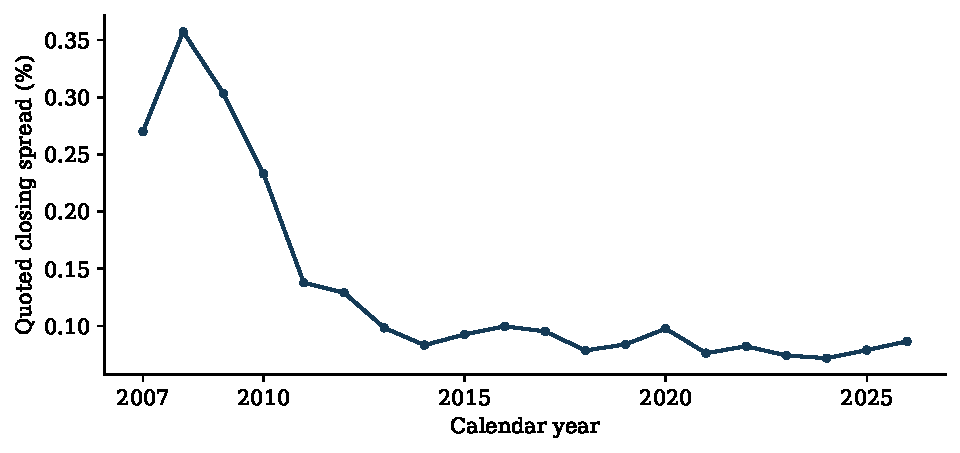
\includegraphics[width=.94\linewidth]{figures/quoted_spread.pdf}
\caption{Annual closing quoted spreads among OMXSB members. These vendor quote measures differ from the effective-spread and execution-cost evidence in Greenwood and Sammon.}
\label{fig:quoted_spread_appendix}
\end{figure}
\begin{figure}[!htbp]\centering
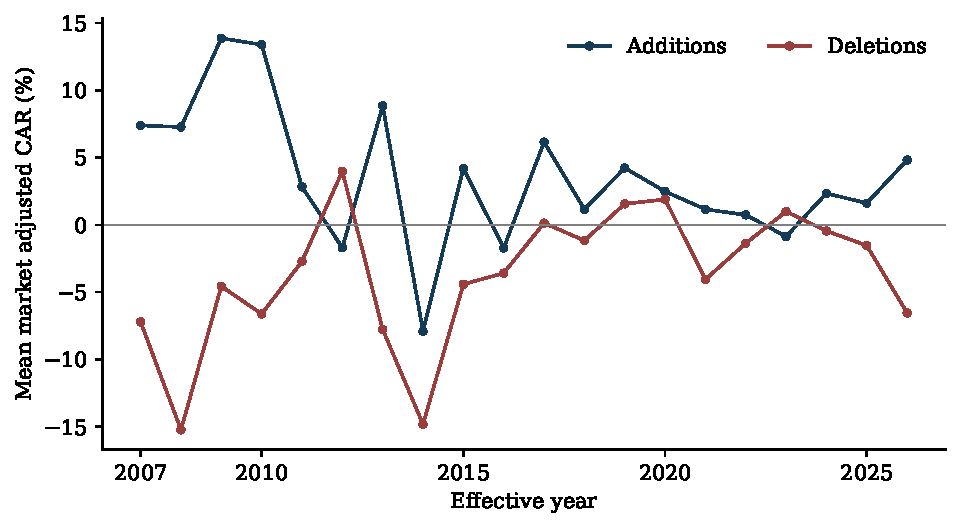
\includegraphics[width=.94\linewidth]{figures/annual_returns.pdf}
\caption{Annual event-return means. Annual averages describe the historical sample; sparse annual review counts limit their precision.}
\label{fig:annual_returns_appendix}
\end{figure}
\FloatBarrier

\section{Reproducibility and disclosure}
\label{app:audit}
\label{app:disclosure}

The analysis is anchored to repository commit \texttt{d2d41666ed21}, with the complete identifier and input hashes in the supporting manifest. Independent reconstruction verifies the main return arithmetic and selected estimators. Rerunning 40 numerical outputs reproduces point estimates and counts; eight differ in simulated inference. Some sparse auxiliary ratio intervals are unstable, so conclusions do not rely on those endpoints. These checks verify specified computations, not every source observation or identifying assumption.

The support package separates frozen estimates from repairs and exploratory additions, and records aggregate results, code, references and unresolved source checks. Licensed security-level data and third-party full texts are not newly redistributed. Reproduction requires authorized access to the documented inputs.

The paper's structure follows the six-part sequence in the BE451 course material. Earlier SSE theses by \citet{fager2024}, \citet{holst2023} and \citet{domeij2021} informed the emphasis on a focused question, a close benchmark study and self-contained exhibits. These examples were examined by Adrien d'Avernas; they are not evidence of an examiner-specific template for Riccardo Sabbatucci. The supporting structure note records the comparison.

\textbf{AI disclosure for this working document.} OpenAI Codex assisted with retrieval, calculations, code review, exhibits and manuscript composition; this prose is AI-generated. An earlier author-supplied draft prepared with Claude informed the narrative revision and was checked claim by claim against the sources and calculations. The BE451 syllabus permits disclosed assistance but prohibits AI directly writing thesis text \citep{sse2026}. This document is a research aid, not a submission-compliant manuscript. The authors must write the submitted prose, verify the findings and disclose assistance accurately.
